\scanpage{129}
\[
\unsure{\mathcal G_{1,1}|\mathfrak S_{1,1}}\simeq\mathcal T_{1,2}^{!}
\qquad
\begin{pmatrix}-1&1\\0&1\end{pmatrix}
\qquad
\rho\left(\unsure{\tfrac12|1},\tfrac12\right)=\left(\tfrac12,-\tfrac12\right)
\]

\figure{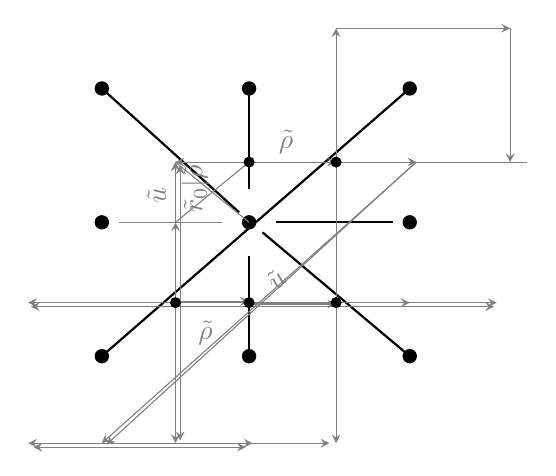
\begin{tikzpicture}[x=0.85cm,y=0.85cm,>=stealth]
\foreach \x in {1.1,3.3,5.7}{\foreach \y in {1.3,3.3,5.3}{\fill (\x,\y) circle (2.6pt);}}
\draw[thick] (1.1,1.3)--(5.7,5.3);
\draw[thick] (1.1,5.3)--(3.15,3.45) (3.5,3.15)--(5.7,1.3);
\draw[thick] (3.3,1.3)--(3.3,2.8) (3.3,3.8)--(3.3,5.3);
\draw[gray] (1.35,3.3)--(2.9,3.3);
\draw[thick] (3.7,3.3)--(5.45,3.3);
\draw[gray,<->] (0,2.1)--(7,2.1);
\draw[gray,<->] (0.04,2.04)--(6.96,2.04);
\draw[gray,->] (2.2,2.12)--(3.3,2.12);
\draw[gray,->] (3.3,2.08)--(4.6,2.08);
\draw[gray,->] (4.6,2.1)--(5.7,2.1);
\draw[gray,<->] (2.2,0)--(2.2,4.2);
\draw[gray,<->] (2.27,0.04)--(2.27,4.15);
\draw[gray,->] (2.2,2.1)--(2.2,3.3);
\draw[gray,->] (2.2,3.3)--(2.2,4.2);
\draw[gray,->] (4.6,4.2)--(4.6,0);
\draw[gray,<->] (0,0)--(4.5,0);
\draw[gray,<->] (0.08,-0.06)--(3.25,-0.06);
\draw[gray,->] (2.2,0)--(3.35,0);
\draw[gray,<->] (2.2,4.2)--(4.6,4.2);
\draw[gray,->] (4.6,4.2)--(5.8,4.2);
\draw[gray] (5.8,4.2)--(7.45,4.2);
\draw[gray,->] (4.6,4.2)--(4.6,6.2);
\draw[gray,->] (4.6,6.2)--(7.2,6.2);
\draw[gray,->] (7.2,6.2)--(7.2,4.2);
\draw[gray,->] (5.8,4.2)--(1.1,0);
\draw[gray,->] (5.75,4.16)--(1.17,-0.02);
\draw[gray] (2.2,4.2)--(3.3,3.3) (2.2,3.3)--(3.3,4.2);
\foreach \p in {(2.2,2.1),(3.3,2.1),(4.6,2.1),(4.6,4.2),(3.3,4.2)}{\fill \p circle (2pt);}
\node[gray,rotate=90] at (1.92,3.7) {$\unsure{\tilde u}$};
\node[gray,rotate=90] at (2.5,3.8) {$\unsure{\tilde r_0|\tilde\rho}$};
\node[gray] at (3.85,4.5) {$\unsure{\tilde\rho}$};
\node[gray] at (2.65,1.65) {$\unsure{\tilde\rho}$};
\node[gray,rotate=45] at (3.7,2.45) {$\unsure{\tilde u}$};
\end{tikzpicture}}

\[
r_0\unsure{u}r_0
\qquad
(ur_1)^{-1}=r_1u^{-1}
\]
\[
(ur_\infty)^{-1}=r_\infty u^{-1}
\]
\[
\tilde v^{-1}\tilde u\tilde v\tilde u^{-1}
\qquad
(ur_\infty)^{-1}
\]
\diagram{\begin{tikzcd}[column sep=large]
\tilde u\tilde v & (vr_\infty)^{-1}\unsure{\circ j|\circ c_j}=r_\infty v^{-1} \arrow[l]
\end{tikzcd}}
\[
\tilde\rho\qquad r_1v^{-1}
\]

\[
(u,\ell)(\unsure{u'},\ell')=(uu',u\ell')\ell
\]
\diagram{\begin{tikzcd}[column sep=large,row sep=large]
& u(a) \arrow[dr,dash] & \\
a \arrow[ur,"\unsure{\ell}"] \arrow[dr,dash,"\ell'"'] \arrow[rr] \arrow[rr,bend left=10,"\deleted{\unsure{u(\ell')}}"] \arrow[rr,bend right=10,"\deleted{\unsure{u'(\ell)}}"'] & & uu'(a)\\
& u'(a) \arrow[ur,dash,"\deleted{\unsure{u(\ell')}}"'] &
\end{tikzcd}}

\[
\begin{aligned}
\ell &: a\longrightarrow ua\\
\ell' &: a\mathbin{-\!\!-}u'a
\end{aligned}
\qquad
\begin{aligned}
u'(\ell)&:u'a\mathbin{-\!\!-}u'ua\\
\uline{u(\ell')}&:\uline{ua\mathbin{-\!\!-}uu'a}
\end{aligned}
\]
\diagram{\begin{tikzcd}
a \arrow[r,dash,"\ell"] & ua \arrow[r,dash] & uu'a
\end{tikzcd}}
\margin{129}
